\section{Misure a frequenza fissa}

In questa sezione si è analizzato il funzionamento (guadagno in tensione, limiti di linearità, eventuali fenomeni di clipping) a frequenza fissa. Si è scelto di operare dunque a $f=\SI{1.031\pm 0.05}{\kHz}$ (frequenza misurata dal frequenzimetro dell'oscilloscopio).\\

\subsection{Common source}
Innanzi tutto si è notato che il circuito sfasa effettivamente il segnale di $\pi$ come
si può notare dall'immagine seguente \ref{f:INV} (acquisita dall'oscilloscopio).

\begin{figure}[h]
	\centering
	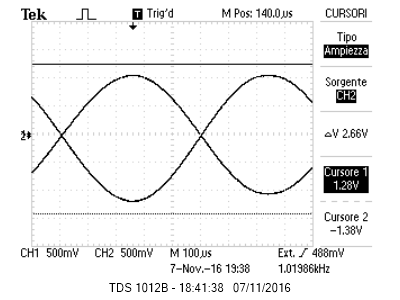
\includegraphics[scale=0.6]{inversion.png}
	\caption{Inversione in configurazione di common source}
	\label{f:INV}
\end{figure}
Si sono poi presi i segnali di input e output con l'oscilloscopio
In configurazione di common source(misurando la tensione sul drain) sono stati ottenuti i dati e il fit riassunti in figura \ref{f:CS} 

\begin{figure}[h]
	\centering
	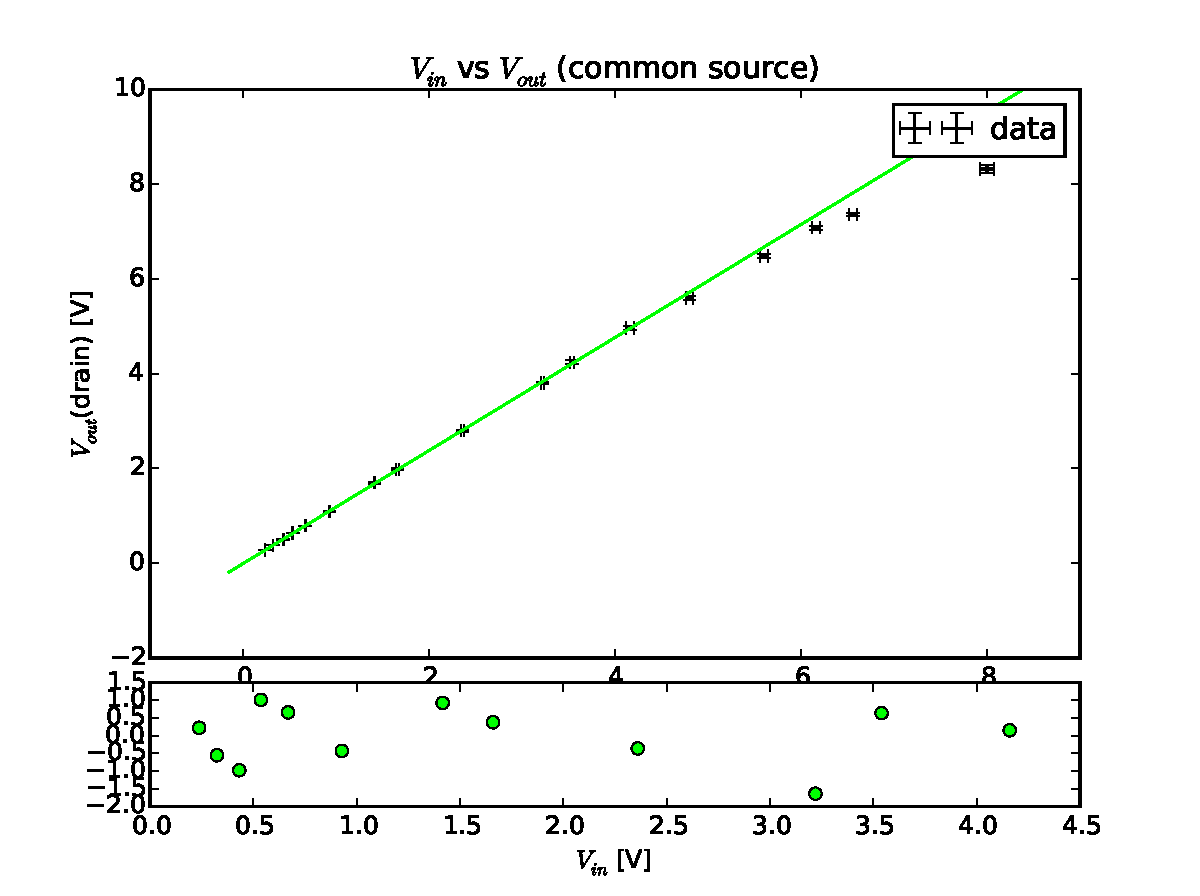
\includegraphics[scale=0.6]{plt_cs.pdf}
	\caption{Piccola tensione di uscita al drain del circuito al variare della tensione (pp) del segnale $V_{in}$}
	\label{f:CS}
\end{figure}

Ovviamente, posto che la linearità si perde a tensioni di ingresso elevate, per poter fittare la retta si è dovuto scegliere un valore di cutoff. Si è scelto di porlo a $\SI{4.5}{V}$. Per il fit, sebbene ci si aspetti di trovare una retta passante per l'origine, si è scelta una retta affine. Sono stati considerati sia gli errori sulle tensioni di ingresso che quelli sulle tensioni di uscita, e sono stati trascurati, per il fit, gli errori di calibrazione.
Sono stati dunque ottenuti questi risultati:\\
$A=1.193\pm 0.006$\\
$V_0=\SI{-0.007 \pm 0.003}{V} $\\
$\rho=-0.78$\\
$\chi^2=7.23$ ($10$ dof, $p = 0.70$)\\
Vi è ancora da aggiungere il contributo dovuto all'errore di calibrazione. Supponendo che gli errori di calibrazione fra le tensioni di ingresso e quelle di uscita siano a loro volta scorrelati, l'errore sistematico su $\sigma_{V_{0}}^2=\sigma_{V_{out}}^2+A^2\sigma_{V_{in}}^2$. Usando come errore sistematico quando riportato nel data-sheet ($3\%+\SI{1}{\mV}$ errore di lettura, mediato sul campione dei misure) si ottiene un errore sistematico di $\SI{2}{\mV}$. Se si sommano in quadratura quest'errore sistematico e l'errore dato dal fit si ottiene $V_0=\SI{-0.007 \pm 0.004}{V}$, compatibile entro 2 sigma con 0.
Si può applicare la stessa procedura ad A. In questo caso per gli errori relativi vale:
$(\delta A)^2=(\delta V_{in})^2+(\delta V_{out})^2=4 \% $. Sommando nuovamente in quadratura quest'errore sistematico a quello dato dal fit si ottiene:\\
$A=1.19\pm 0.04$\\
Si nota come, in questo caso, l'errore sistematico sia tutt'altro che trascurabile.\\ 
Si devono confrontare i valori misurati con quanto atteso. Usando il valore di transconduttanza misurato in precedenza e il valore di resistenza del trimmer di $\SI{227\pm 3}{\ohm}$ si ottiene un'amplificazione attesa di:
$A=-\frac{g_mR_1}{1+g_mR_2}= 1.213\pm 0.018$\\
compatibile con quanto atteso.

Per quanto riguarda l'uscita dalla linearità essa è evidente dal grafico fin sopra i $\SI{4.5}{\V}$, palesata ancor di più dal clipping visibile in \ref{f:CLICS}.

\begin{figure}[h]
	\centering
	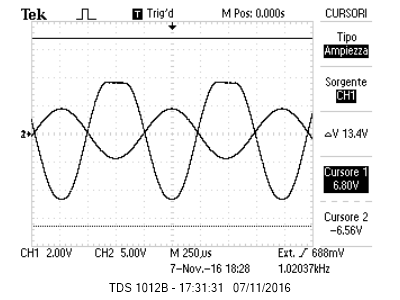
\includegraphics[scale=0.6]{clipup.png}
	\caption{Clipping del segnale in configurazione common source. Come ci si può aspettare si vede nella parte alta del segnale}
	\label{f:CLICS}
\end{figure}



\subsection{Source follower}
Procedendo similmente a quanto fatto per la configurazione di common source, si sono ottenuti i dati e il fit riassunto nella figura \ref{f:SF}. Per il fit, sempre di una retta affine, si è scelto un cutoff di $\SI{5}{V}$. Si sono ottenuti i seguenti parametri:\\
$A=0.467\pm 0.002$\\
$V_0=\SI{0.0025 \pm 0.0011}{V} $\\
$\rho=-0.75$\\
$\chi^2=14.76$ ($11$ dof, $p = 0.19$)\\

Anche qui sono da aggiungere gli errori sistematici. Si sono ottenuti i valori di:\\
$V_0=\SI{0.003 \pm 0.002}{V} $\\ 
$A=0.47\pm 0.01$ \\

Anche qui questi valori vanno confrontati con i valori attesi:\\
$A=\frac{g_mR_2}{1+g_mR_2}=0.500 \pm 0.006$\\
Si ha dunque un discreto disaccordo con i il valore atteso.

\begin{figure}[h]
	\centering
	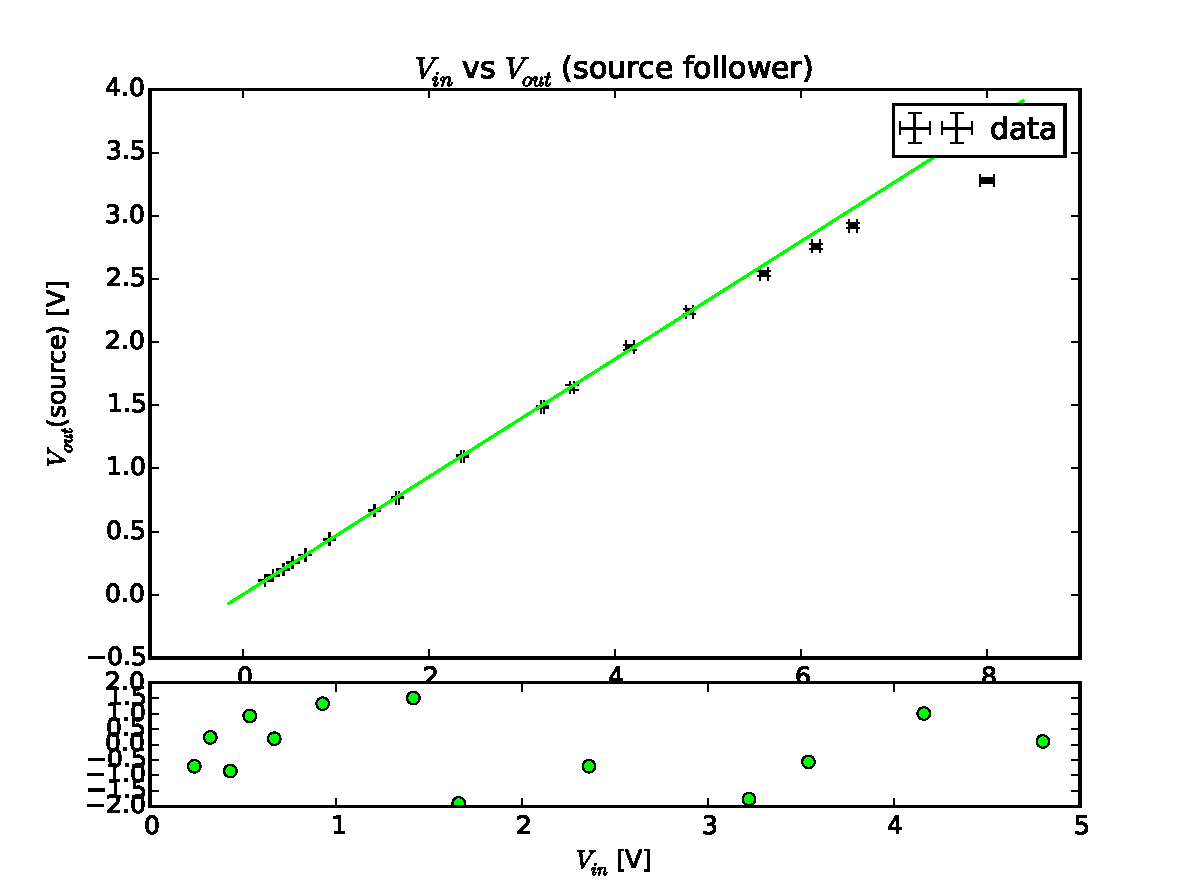
\includegraphics[scale=0.6]{plt_sf.pdf}
	\caption{Piccola tensione di uscita al source del circuito al variare della tensione (pp) del segnale $V_{in}$}
	\label{f:SF}
\end{figure}

Anche in questo grafico è evidente il clipping \ref{f:CLICF1}

\begin{figure}[h]
	\centering
	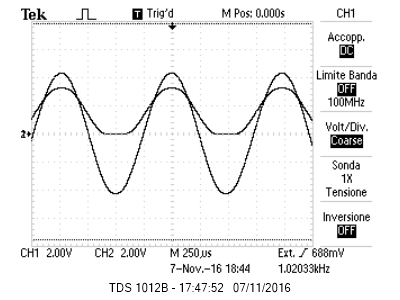
\includegraphics[scale=0.6]{clipsource2.png}
	\caption{Clipping del segnale in configurazione source follower. Si nota inoltre come il segnale non sia invertito}
	\label{f:CLICF1}
\end{figure}



%\newcommand{\comment}[1]{}


%Common source
%[ 1.19258003 -0.00728627]
%0.00562855935642
%0.0029181504972
%-0.77681826835
%ChiSquare = 7.229061209357948 (10 DoF, p = 0.7036576593491565)
%
%Source follower
%[ 0.46571661  0.00252217]
%0.00205837208081
%0.00111885248818
%-0.749519956342
%ChiSquare = 14.758774254692398 (11 DoF, p = 0.1938088526493881)
